% GNUPLOT: LaTeX picture with Postscript
\begingroup
  \makeatletter
  \providecommand\color[2][]{%
    \GenericError{(gnuplot) \space\space\space\@spaces}{%
      Package color not loaded in conjunction with
      terminal option `colourtext'%
    }{See the gnuplot documentation for explanation.%
    }{Either use 'blacktext' in gnuplot or load the package
      color.sty in LaTeX.}%
    \renewcommand\color[2][]{}%
  }%
  \providecommand\includegraphics[2][]{%
    \GenericError{(gnuplot) \space\space\space\@spaces}{%
      Package graphicx or graphics not loaded%
    }{See the gnuplot documentation for explanation.%
    }{The gnuplot epslatex terminal needs graphicx.sty or graphics.sty.}%
    \renewcommand\includegraphics[2][]{}%
  }%
  \providecommand\rotatebox[2]{#2}%
  \@ifundefined{ifGPcolor}{%
    \newif\ifGPcolor
    \GPcolorfalse
  }{}%
  \@ifundefined{ifGPblacktext}{%
    \newif\ifGPblacktext
    \GPblacktexttrue
  }{}%
  % define a \g@addto@macro without @ in the name:
  \let\gplgaddtomacro\g@addto@macro
  % define empty templates for all commands taking text:
  \gdef\gplbacktext{}%
  \gdef\gplfronttext{}%
  \makeatother
  \ifGPblacktext
    % no textcolor at all
    \def\colorrgb#1{}%
    \def\colorgray#1{}%
  \else
    % gray or color?
    \ifGPcolor
      \def\colorrgb#1{\color[rgb]{#1}}%
      \def\colorgray#1{\color[gray]{#1}}%
      \expandafter\def\csname LTw\endcsname{\color{white}}%
      \expandafter\def\csname LTb\endcsname{\color{black}}%
      \expandafter\def\csname LTa\endcsname{\color{black}}%
      \expandafter\def\csname LT0\endcsname{\color[rgb]{1,0,0}}%
      \expandafter\def\csname LT1\endcsname{\color[rgb]{0,1,0}}%
      \expandafter\def\csname LT2\endcsname{\color[rgb]{0,0,1}}%
      \expandafter\def\csname LT3\endcsname{\color[rgb]{1,0,1}}%
      \expandafter\def\csname LT4\endcsname{\color[rgb]{0,1,1}}%
      \expandafter\def\csname LT5\endcsname{\color[rgb]{1,1,0}}%
      \expandafter\def\csname LT6\endcsname{\color[rgb]{0,0,0}}%
      \expandafter\def\csname LT7\endcsname{\color[rgb]{1,0.3,0}}%
      \expandafter\def\csname LT8\endcsname{\color[rgb]{0.5,0.5,0.5}}%
    \else
      % gray
      \def\colorrgb#1{\color{black}}%
      \def\colorgray#1{\color[gray]{#1}}%
      \expandafter\def\csname LTw\endcsname{\color{white}}%
      \expandafter\def\csname LTb\endcsname{\color{black}}%
      \expandafter\def\csname LTa\endcsname{\color{black}}%
      \expandafter\def\csname LT0\endcsname{\color{black}}%
      \expandafter\def\csname LT1\endcsname{\color{black}}%
      \expandafter\def\csname LT2\endcsname{\color{black}}%
      \expandafter\def\csname LT3\endcsname{\color{black}}%
      \expandafter\def\csname LT4\endcsname{\color{black}}%
      \expandafter\def\csname LT5\endcsname{\color{black}}%
      \expandafter\def\csname LT6\endcsname{\color{black}}%
      \expandafter\def\csname LT7\endcsname{\color{black}}%
      \expandafter\def\csname LT8\endcsname{\color{black}}%
    \fi
  \fi
  \setlength{\unitlength}{0.0500bp}%
  \begin{picture}(8502.00,5668.00)%
    \gplgaddtomacro\gplbacktext{%
      \csname LTb\endcsname%
      \put(946,704){\makebox(0,0)[r]{\strut{} 0.2}}%
      \csname LTb\endcsname%
      \put(946,1134){\makebox(0,0)[r]{\strut{} 0.4}}%
      \csname LTb\endcsname%
      \put(946,1565){\makebox(0,0)[r]{\strut{} 0.6}}%
      \csname LTb\endcsname%
      \put(946,1995){\makebox(0,0)[r]{\strut{} 0.8}}%
      \csname LTb\endcsname%
      \put(946,2425){\makebox(0,0)[r]{\strut{} 1}}%
      \csname LTb\endcsname%
      \put(946,2856){\makebox(0,0)[r]{\strut{} 1.2}}%
      \csname LTb\endcsname%
      \put(946,3286){\makebox(0,0)[r]{\strut{} 1.4}}%
      \csname LTb\endcsname%
      \put(946,3716){\makebox(0,0)[r]{\strut{} 1.6}}%
      \csname LTb\endcsname%
      \put(946,4146){\makebox(0,0)[r]{\strut{} 1.8}}%
      \csname LTb\endcsname%
      \put(946,4577){\makebox(0,0)[r]{\strut{} 2}}%
      \csname LTb\endcsname%
      \put(946,5007){\makebox(0,0)[r]{\strut{} 2.2}}%
      \csname LTb\endcsname%
      \put(1231,484){\makebox(0,0){\strut{} 5}}%
      \csname LTb\endcsname%
      \put(1536,484){\makebox(0,0){\strut{} 7}}%
      \csname LTb\endcsname%
      \put(1842,484){\makebox(0,0){\strut{} 9}}%
      \csname LTb\endcsname%
      \put(2147,484){\makebox(0,0){\strut{} 11}}%
      \csname LTb\endcsname%
      \put(2453,484){\makebox(0,0){\strut{} 13}}%
      \csname LTb\endcsname%
      \put(2758,484){\makebox(0,0){\strut{} 15}}%
      \csname LTb\endcsname%
      \put(3064,484){\makebox(0,0){\strut{} 17}}%
      \csname LTb\endcsname%
      \put(3369,484){\makebox(0,0){\strut{} 19}}%
      \csname LTb\endcsname%
      \put(3675,484){\makebox(0,0){\strut{} 21}}%
      \csname LTb\endcsname%
      \put(3980,484){\makebox(0,0){\strut{} 23}}%
      \csname LTb\endcsname%
      \put(4286,484){\makebox(0,0){\strut{} 25}}%
      \csname LTb\endcsname%
      \put(4592,484){\makebox(0,0){\strut{} 27}}%
      \csname LTb\endcsname%
      \put(4897,484){\makebox(0,0){\strut{} 29}}%
      \csname LTb\endcsname%
      \put(5203,484){\makebox(0,0){\strut{} 31}}%
      \csname LTb\endcsname%
      \put(5508,484){\makebox(0,0){\strut{} 33}}%
      \csname LTb\endcsname%
      \put(5814,484){\makebox(0,0){\strut{} 35}}%
      \csname LTb\endcsname%
      \put(6119,484){\makebox(0,0){\strut{} 37}}%
      \csname LTb\endcsname%
      \put(6425,484){\makebox(0,0){\strut{} 39}}%
      \csname LTb\endcsname%
      \put(6730,484){\makebox(0,0){\strut{} 41}}%
      \csname LTb\endcsname%
      \put(7036,484){\makebox(0,0){\strut{} 43}}%
      \csname LTb\endcsname%
      \put(7341,484){\makebox(0,0){\strut{} 45}}%
      \csname LTb\endcsname%
      \put(7647,484){\makebox(0,0){\strut{} 47}}%
      \csname LTb\endcsname%
      \put(7952,484){\makebox(0,0){\strut{} 49}}%
      \put(176,2855){\rotatebox{-270}{\makebox(0,0){\strut{}transfer rate in GB per second}}}%
      \put(4591,154){\makebox(0,0){\strut{}number of nodes}}%
      \put(4591,5337){\makebox(0,0){\strut{}Data distribution, HPC cluster. 224 GB of pair-ended FASTQ files}}%
    }%
    \gplgaddtomacro\gplfronttext{%
      \csname LTb\endcsname%
      \put(1210,4834){\makebox(0,0)[l]{\strut{}without striping}}%
      \csname LTb\endcsname%
      \put(1210,4614){\makebox(0,0)[l]{\strut{}striped1}}%
      \csname LTb\endcsname%
      \put(1210,4394){\makebox(0,0)[l]{\strut{}striped2}}%
      \csname LTb\endcsname%
      \put(1210,4174){\makebox(0,0)[l]{\strut{}striped3}}%
      \csname LTb\endcsname%
      \put(1210,3954){\makebox(0,0)[l]{\strut{}striped4}}%
    }%
    \gplbacktext
    \put(0,0){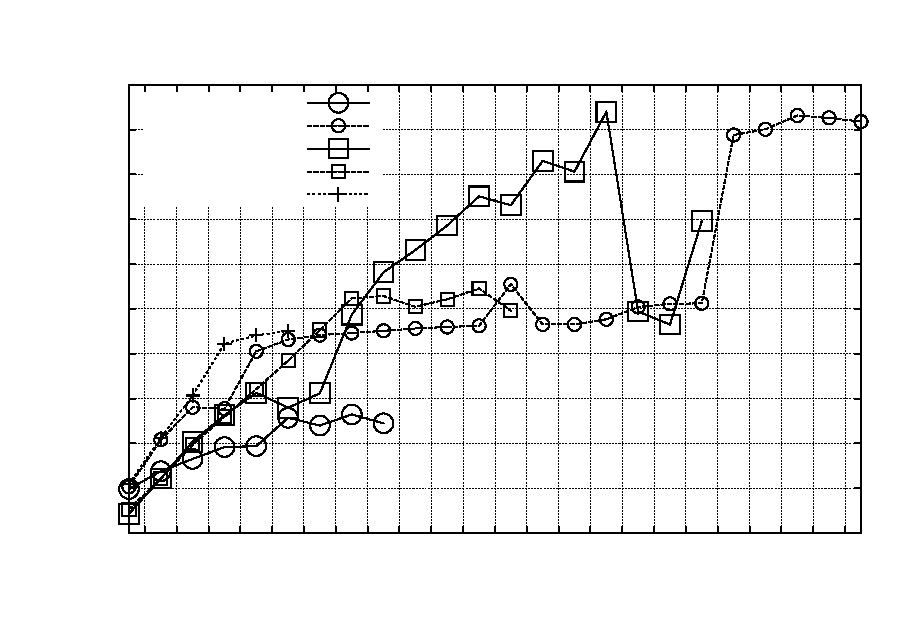
\includegraphics{fig}}%
    \gplfronttext
  \end{picture}%
\endgroup
